% =====================================================================
% Short paper - Preços do dia a dia nos EUA (2015-2026)
% Aluno: João Gabriel Tavares Silva - Matrícula 221021071 - UnB
% Classe abnTeX2 (ABNT NBR 6022:2018 - artigo científico)
% Compilar com pdfLaTeX + BibTeX (padrão do Overleaf)
% =====================================================================
\documentclass[
  article,            % artigo acadêmico
  12pt,
  oneside,
  a4paper,
  section=TITLE,      % seções primárias em maiúsculas
  english,            % idioma adicional (abstract)
  brazil              % idioma principal
]{abntex2}

\usepackage[T1]{fontenc}
\usepackage[utf8]{inputenc}
\usepackage{times}              % fonte Times (ABNT)
\usepackage{indentfirst}
\usepackage{graphicx}
\usepackage{microtype}
\usepackage{booktabs}
\usepackage{tabularx}
\usepackage{float}
\usepackage{amsmath}
\usepackage[alf]{abntex2cite}   % citações autor-data (ABNT NBR 10520)

\graphicspath{{figuras/}}

% ---------- Dados do documento ----------
\titulo{Preços do dia a dia nos EUA (2015--2026): inflação real e correlações entre pares de itens}
\tituloestrangeiro{Everyday prices in the US (2015--2026): real inflation and pairwise correlations between items}
\autor{João Gabriel Tavares Silva}
\local{Brasília}
\data{2026}

\makeatletter
\hypersetup{
  pdftitle={\@title},
  pdfauthor={\@author},
  pdfsubject={Short paper - análise de preços médios do BLS},
  colorlinks=true, linkcolor=black, citecolor=black, urlcolor=blue
}
\makeatother

% ---------- Layout ABNT ----------
\setlrmarginsandblock{3cm}{2cm}{*}
\setulmarginsandblock{3cm}{2cm}{*}
\checkandfixthelayout
\setlength{\parindent}{1.25cm}
\setlength{\parskip}{0.2cm}
\OnehalfSpacing

% Títulos em Times negrito (seções primárias em maiúsculas pela opção section=TITLE)
\renewcommand{\ABNTEXchapterfont}{\rmfamily\bfseries}
\renewcommand{\ABNTEXchapterfontsize}{\normalsize}
\renewcommand{\ABNTEXsectionfont}{\rmfamily\bfseries}
\renewcommand{\ABNTEXsectionfontsize}{\normalsize}
\renewcommand{\ABNTEXsubsectionfont}{\rmfamily\bfseries}
\renewcommand{\ABNTEXsubsectionfontsize}{\normalsize}

% Tabelas: texto menor e espaçamento simples
\newcommand{\tabelaabnt}{\footnotesize\SingleSpacing}

\begin{document}
\selectlanguage{brazil}
\frenchspacing
\renewcommand{\resumoname}{RESUMO}
\renewcommand{\bibname}{REFERÊNCIAS}
\renewcommand{\refname}{REFERÊNCIAS}

% ---------- Cabeçalho com logo da UnB ----------
\begin{center}
  
\includegraphics[width=2.6cm]{logo-unb}\\[0.4cm]
  {\large\bfseries Preços do dia a dia nos EUA (2015--2026): inflação real e correlações entre pares de itens\par}
  \vspace{0.4cm}
  {\normalsize João Gabriel Tavares Silva\par}
  {\small Universidade de Brasília (UnB) $\cdot$ Matrícula: 221021071\par}
\end{center}
\vspace{0.2cm}

% ---------- Resumo ----------
\begin{resumoumacoluna}
  \SingleSpacing
  Este trabalho analisa os preços médios mensais de 74 itens de consumo nos Estados Unidos entre janeiro de 2015 e julho de 2026, publicados pelo Bureau of Labor Statistics (BLS). Corrigidos os problemas encontrados na base e deflacionados os preços pelo CPI-U (+38,5\% no período), todos os 62 itens com dados suficientes ficaram mais caros em dólares correntes, mas só 35 subiram acima da inflação. Entre os 1.891 pares de itens, 86\% têm $|r| > 0{,}5$ quando se comparam níveis de preço, contra 3\% quando se comparam variações mensais dessazonalizadas: a maior parte da associação aparente é tendência comum. As relações robustas ficam dentro de uma mesma cadeia produtiva. A inflação do diesel antecede a dos alimentos em cerca de cinco meses ($r = 0{,}51$), mas a precedência estatística é fraca.

  \vspace{0.5\onelineskip}
  \noindent
  \textbf{Palavras-chave}: preços ao consumidor; inflação; correlação espúria; causalidade de Granger.
\end{resumoumacoluna}

\renewcommand{\resumoname}{ABSTRACT}
\begin{resumoumacoluna}
  \SingleSpacing
  \begin{otherlanguage*}{english}
    This paper analyzes the monthly average prices of 74 consumer items in the United States from January 2015 to July 2026, published by the Bureau of Labor Statistics (BLS). After correcting the problems found in the dataset and deflating prices by the CPI-U (+38.5\% over the period), all 62 items with sufficient data became more expensive in current dollars, but only 35 rose faster than inflation. Across the 1,891 pairs of items, 86\% show $|r| > 0.5$ when price levels are compared, against 3\% when deseasonalized monthly changes are compared: most of the apparent association is a common trend. Robust relationships stay within the same supply chain. Diesel inflation leads food inflation by about five months ($r = 0.51$), but statistical precedence is weak.

    \vspace{0.5\onelineskip}
    \noindent
    \textbf{Keywords}: consumer prices; inflation; spurious correlation; Granger causality.
  \end{otherlanguage*}
\end{resumoumacoluna}

\textual

% =====================================================================
\section{Introdução}

O choque inflacionário de 2021--2022 recolocou no debate público o custo de itens básicos como ovos, carne, leite e gasolina. Índices agregados, como o CPI, mostram a inflação média, mas escondem trajetórias muito diferentes entre produtos. A série de preços médios do BLS permite olhar item a item, em dólares, e por isso circula amplamente em bases públicas como o Kaggle.

O trabalho responde a três perguntas: quais itens ficaram mais caros acima da inflação geral; quais pares de itens se movem juntos depois de removida a tendência comum; e se o preço da energia antecipa o preço dos alimentos. O código completo, interativo e reproduzível está em um notebook público \cite{silva2026precos} (\href{https://github.com/joaogabrielts0611-ai/Trabalho---PSP3-Joao-Gabriel-Tavares}{GitHub} $\cdot$ \href{https://colab.research.google.com/github/joaogabrielts0611-ai/Trabalho---PSP3-Joao-Gabriel-Tavares/blob/main/analise_precos_eua.ipynb}{Google Colab}).

% =====================================================================
\section{Revisão de literatura}

Correlacionar séries de preços exige cuidado conhecido há quase um século. \citeonline{yule1926} mostrou que séries temporais com tendência produzem correlações altas sem qualquer relação entre os fenômenos, as chamadas correlações sem sentido. \citeonline{granger1974} levaram o problema às regressões econométricas: com séries não estacionárias, o $R^2$ e as estatísticas $t$ indicam relação onde não há, e a recomendação é trabalhar com variações. Preços ao consumidor são o caso típico, porque compartilham a inflação geral.

A transmissão de energia para alimentos tem literatura própria. \citeonline{baffes2007} estimou que altas do petróleo se transmitem aos preços internacionais de \textit{commodities} agrícolas, com elasticidade de cerca de 0,18 para alimentos. Para o varejo americano, porém, \citeonline{baumeister2014} não encontraram evidência de que choques do petróleo tenham elevado de forma relevante os preços dos alimentos depois de 2006. A precedência temporal entre as séries costuma ser testada pela causalidade de \citeonline{granger1969}, que mede se o passado de uma série melhora a previsão de outra, sem implicar causalidade econômica, com erros-padrão robustos à autocorrelação \cite{newey1987}.

Choques de oferta também criam correlações temporárias. \citeonline{lusk2021} documentaram que o fechamento de frigoríficos na primavera de 2020 elevou ao mesmo tempo os preços de carne bovina e suína no varejo, enquanto o preço pago ao produtor caía. Por fim, quando milhares de correlações são testadas ao mesmo tempo, o controle da taxa de falsas descobertas \cite{benjamini1995} evita que pares significativos por acaso sejam tomados como achados.

% =====================================================================
\section{Metodologia}

A base reúne 8.869 observações item-mês de 74 itens (carnes, laticínios, hortifrúti, grãos, bebidas e energia), com preço médio nacional sem ajuste sazonal, de jan./2015 a jul./2026 \cite{bls2026}. O deflator é o CPI-U, todos os itens, sem ajuste sazonal \cite{fred2026}; outubro de 2025, não publicado por causa da paralisação do governo americano, foi interpolado.

Uma auditoria da base contra o resumo que a acompanha encontrou seis problemas, corrigidos antes da análise: café e batata chips em categorias erradas (reclassificação em 8 grupos); janelas de comparação que eram as 12 primeiras observações, e não os 12 primeiros meses (substituídas por janelas de calendário, 2015 contra ago./2025--jul./2026); séries iniciadas em anos diferentes na mesma mediana (taxa anual equivalente); séries ativas marcadas como descontinuadas (critério de cobertura, resultando em 62 séries); inflação do período informada como cerca de 35\% (CPI-U oficial: +38,5\%); e base dos ovos em ano de gripe aviária (comparação adicional contra 2016--2019).

A variação de cada item compara as médias das janelas inicial e final, o que neutraliza a sazonalidade; a variação real usa preços deflacionados mês a mês. Índices de grupo são médias geométricas dos preços relativos. As correlações entre os 1.891 pares foram calculadas em três transformações: nível do preço, variação em 12 meses e variação mensal do logaritmo do preço dessazonalizada. A terceira é a medida principal, pelos motivos da seção anterior, com p-valores corrigidos por \citeonline{benjamini1995} e robustez verificada por Spearman e pela exclusão de mar.--ago./2020. Para energia e alimentos, usaram-se correlação cruzada com defasagens de 0 a 12 meses, teste de Granger com seis defasagens e regressão com erros de Newey-West.

% =====================================================================
\section{Resultados encontrados}

Os 62 itens subiram em dólares correntes, com mediana de +42\%. Descontada a inflação, só 35 subiram acima do CPI-U, e a mediana real cai para +3,8\%. Os maiores ganhos reais foram do café (+43\%) e do refrigerante em lata (+30\%); as maiores quedas, do macarrão ($-$28\%) e do limão ($-$26\%). Carne bovina, bebidas e energia ganharam da inflação; aves, ovos e laticínios perderam (Tabela~\ref{tab:grupos}). Os ovos mostram o risco de um período-base mal escolhido: contra 2015, ano de gripe aviária, a alta é de 6\%; contra 2016--2019, de 67\%.

\begin{table}[htbp]
  \centering
  \caption{Variação de preços por grupo, 2015 $\rightarrow$ ago./2025--jul./2026 (medianas)}
  \label{tab:grupos}
  \tabelaabnt
  \begin{tabular}{lcccc}
    \toprule
    \textbf{Grupo} & \textbf{Itens} & \textbf{Nominal} & \textbf{Real} & \textbf{Acima da inflação} \\
    \midrule
    Carne bovina & 12 & +57,8\% & +13,8\% & 11 de 12 \\
    Bebidas e café & 5 & +46,5\% & +12,4\% & 4 de 5 \\
    Energia & 8 & +54,6\% & +11,5\% & 8 de 8 \\
    Grãos, padaria e mercearia & 9 & +36,6\% & $-$1,1\% & 4 de 9 \\
    Hortifrúti & 10 & +31,1\% & $-$5,5\% & 5 de 10 \\
    Suínos e frios & 7 & +25,9\% & $-$9,1\% & 1 de 7 \\
    Laticínios & 7 & +21,0\% & $-$12,7\% & 2 de 7 \\
    Aves e ovos & 4 & +15,9\% & $-$16,4\% & 0 de 4 \\
    \bottomrule
  \end{tabular}
  \fonte{Elaboração própria a partir de \citeonline{bls2026} e \citeonline{fred2026}.}
\end{table}

A alta real não foi gradual (Figura~\ref{fig:indices}). Entre 2015 e 2019, quase todos os grupos perderam para a inflação; no choque de 2020--2022, todos ganharam; depois de 2023, só a carne bovina manteve alta real forte (+6,1\% a.a.). As carnes chegaram primeiro ao pico da inflação em 12 meses (nov./2021), a energia em jun./2022 e os alimentos mais processados por último.

\begin{figure}[htbp]
  \centering
  \caption{Índices de preço por grupo e CPI-U (média de 2015 = 100)}
  \label{fig:indices}
  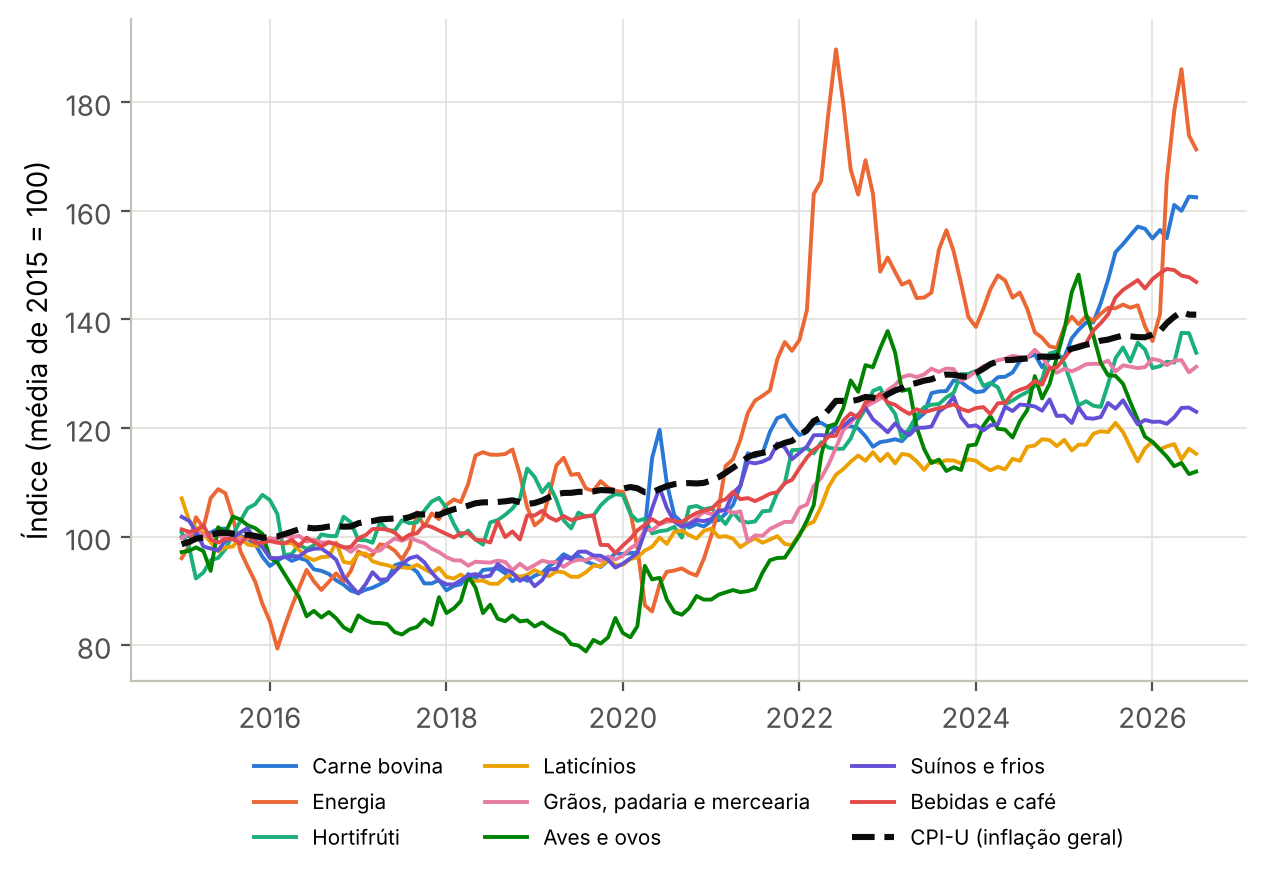
\includegraphics[width=0.82\textwidth]{fig1_indices}
  \fonte{Elaboração própria a partir de \citeonline{bls2026} e \citeonline{fred2026}.}
\end{figure}

Nas correlações, a medida escolhida muda o resultado mais do que qualquer outra decisão (Figura~\ref{fig:correlacoes}). Em nível de preço, a correlação média entre pares é 0,72 e 86\% dos pares têm $|r| > 0{,}5$; em variação mensal dessazonalizada, a média cai para 0,06 e só 3\% passam de 0,5. Refrigerante em lata e cookies, por exemplo, têm $r = 0{,}97$ em nível e $-0{,}02$ em variação mensal, como prevê \citeonline{granger1974}.

\begin{figure}[htbp]
  \centering
  \caption{Distribuição das correlações entre os 1.891 pares, por medida}
  \label{fig:correlacoes}
  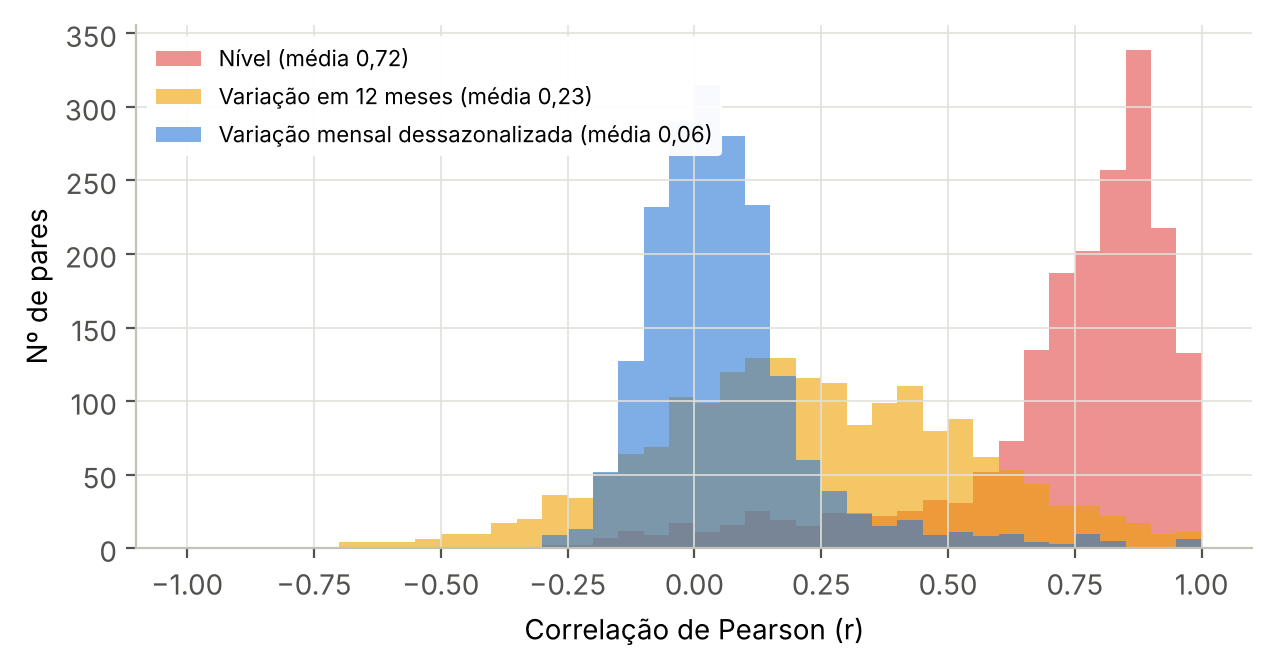
\includegraphics[width=0.82\textwidth]{fig2_correlacoes}
  \fonte{Elaboração própria a partir de \citeonline{bls2026}.}
\end{figure}

Após a correção FDR, 170 pares (9\%) são significativos em variação mensal. Os mais fortes são de uma mesma cadeia: as gasolinas entre si ($r \approx 1{,}00$), diesel e gasolina (0,79) e os cortes bovinos (0,63 a 0,88). Entre grupos, o par mais forte liga costeletas suínas e carne moída ($r = 0{,}53$), mas cai para 0,30 sem mar.--ago./2020, o episódio dos frigoríficos descrito por \citeonline{lusk2021}. O primeiro componente principal explica 14,7\% da variação mensal, contra 4,9\% esperados com itens independentes: o fator comum existe, mas é fraco.

Em variação de 12 meses, a correlação entre diesel e alimentos é máxima com cinco meses de defasagem ($r = 0{,}51$), e a da gasolina, com seis ($r = 0{,}56$). Na regressão, 10\% de alta no diesel acompanham 0,8 ponto percentual a mais de inflação de alimentos, mas sem significância a 5\% com erros de Newey-West ($p = 0{,}078$). No teste de Granger, só 2 das 16 combinações combustível $\times$ grupo passam após a correção FDR. A correlação entre os índices de alimentos e de energia foi de $-$0,37 até 2021 e de +0,19 a partir de 2022: a ligação existe no choque, mas não é estável, o que aproxima o resultado de \citeonline{baumeister2014} mais do que de \citeonline{baffes2007}.

% =====================================================================
\section{Conclusão}

Entre 2015 e 2026, os 62 itens analisados subiram em média 42\% em dólares, mas só 35 ganharam da inflação de 38,5\%; carne bovina e café são as exceções persistentes. As associações entre preços são muito menores do que parecem: em variação mensal dessazonalizada, só 3\% dos pares têm $|r| > 0{,}5$, e os fortes pertencem à mesma cadeia produtiva ou ao mesmo choque. A energia antecede os alimentos em cinco a seis meses, mas de forma fraca e concentrada em 2021--2022.

O trabalho tem limitações: os preços são médias nacionais, que escondem diferenças entre regiões e marcas; o deflator é o CPI-U geral, não o de alimentos; e Granger mede precedência, não causalidade. Ainda assim, a lição de método é direta: antes de qualquer ranking com esta base, é preciso corrigir as janelas de comparação, deflacionar os preços e trabalhar com variações, não com níveis.

% ---------- Referências ----------
\postextual
\bibliography{referencias}

\end{document}
